% Use this template to write your solutions to COS 423 problem sets

\documentclass[12pt]{article}
\usepackage[utf8]{inputenc}
\usepackage{amsmath, amsfonts, amsthm, amssymb, algorithm, graphicx, mathtools, xfrac}
\usepackage[noend]{algpseudocode}
\usepackage{fancyhdr, lastpage}
\usepackage{booktabs}
\usepackage{multirow}
\usepackage{graphicx}
\usepackage{pgfplots}
\usepackage[vmargin=1.20in,hmargin=1.25in,centering,letterpaper]{geometry}
\setlength{\headsep}{.50in}
\setlength{\headheight}{15pt}

% Landau notation
\DeclareMathOperator{\BigOm}{\mathcal{O}}
\newcommand{\BigOh}[1]{\BigOm\left({#1}\right)}
\DeclareMathOperator{\BigTm}{\Theta}
\newcommand{\BigTheta}[1]{\BigTm\left({#1}\right)}
\DeclareMathOperator{\BigWm}{\Omega}
\newcommand{\BigOmega}[1]{\BigWm\left({#1}\right)}
\DeclareMathOperator{\LittleOm}{\mathrm{o}}
\newcommand{\LittleOh}[1]{\LittleOm\left({#1}\right)}
\DeclareMathOperator{\LittleWm}{\omega}
\newcommand{\LittleOmega}[1]{\LittleWm\left({#1}\right)}

% argmin and argmax
\newcommand{\argmin}{\operatornamewithlimits{argmin}}
\newcommand{\argmax}{\operatornamewithlimits{argmax}}

\newcommand{\calP}{\mathcal{P}}
\newcommand{\Z}{\mathbb{Z}}
\newcommand{\R}{\mathbb{R}}
\newcommand{\Exp}{\mathbb{E}}
\newcommand{\Q}{\mathbb{Q}}
\newcommand{\sign}{\mathrm{sign\ }}
\newcommand{\abs}{\mathrm{abs\ }}
\newcommand{\eps}{\varepsilon}
\newcommand{\zo}{\{0, 1\}}
\newcommand{\SAT}{\mathit{SAT}}
\renewcommand{\P}{\mathbf{P}}
\newcommand{\NP}{\mathbf{NP}}
\newcommand{\coNP}{\co{NP}}
\newcommand{\co}[1]{\mathbf{co#1}}
\renewcommand{\Pr}{\mathop{\mathrm{Pr}}}

% theorems, lemmas, invariants, etc.
\newtheorem{theorem}{Theorem}
\newtheorem{lemma}[theorem]{Lemma}
\newtheorem{invariant}[theorem]{Invariant}
\newtheorem{corollary}[theorem]{Corollary}
\newtheorem{definition}[theorem]{Definition}
\newtheorem{property}[theorem]{Property}
\newtheorem{proposition}[theorem]{Proposition}

% piecewise functions
\newenvironment{piecewise}{\left \{\begin{array}{l@{,\ }l}}
{\end{array}\right.}

% paired delimiters
\DeclarePairedDelimiter{\ceil}{\lceil}{\rceil}
\DeclarePairedDelimiter{\floor}{\lfloor}{\rfloor}
\DeclarePairedDelimiter{\len}{|}{|}
\DeclarePairedDelimiter{\set}{\{}{\}}

\makeatletter
\@addtoreset{equation}{section}
\makeatother
\renewcommand{\theequation}{\arabic{section}.\arabic{equation}}

% algorithms
\algnewcommand\algorithmicinput{\textbf{INPUT:}}
\algnewcommand\INPUT{\item[\algorithmicinput]}
\algnewcommand\algorithmicoutput{\textbf{OUTPUT:}}
\algnewcommand\OUTPUT{\item[\algorithmicoutput]}


% Formating Macros

\pagestyle{fancy}
\lhead{\sc \hmwkClass\ $\; \;\cdot \; \;$ \hmwkSemester\ $\; \;\cdot \; \;$
Problem \hmwkAssignmentNum.\hmwkProblemNum}
%\chead{\sc Problem \hmwkAssignmentNum.\hmwkProblemNum}
%\chead{}
\rhead{\em \hmwkAuthorName\ $($\hmwkAuthorID$)$\/}
\cfoot{}
\lfoot{}
\rfoot{\sc Page\ \thepage\ of\ \protect\pageref{LastPage}}
\renewcommand\headrulewidth{0.4pt}
\renewcommand\footrulewidth{0.4pt}

\fancypagestyle{fancycollab}
{
    \lfoot{\textit{Collaborators: \hmwkCollaborators}}
}

\fancypagestyle{problemstatement}
{
    \rhead{}
    \lfoot{}
}

%%%%%% Begin document with header and title %%%%%%%%%%%%%%%%%%%%%%%%%

\begin{document}

%%%%%% Header Information %%%%%%%%%%%%%%%%%%%%%%%%%%%%%%%%%%%%%%%%%%%

%%% Shouldn't need to change these
\newcommand{\hmwkClass}{COS 255}
\newcommand{\hmwkSemester}{Spring 2016}

%%% Your name, in standard First Last format
\newcommand{\hmwkAuthorName}{Lukas Leung}
%%% Your NetID
\newcommand{\hmwkAuthorID}{lleung}

%%% The problem set number (just the number)
\newcommand{\hmwkAssignmentNum}{6}

%%% The problem number (just the number)
\newcommand{\hmwkProblemNum}{0}

%%% A list of your collaborators' NetIDs, separated by ", ".
%%% You can use a new line ("\\") in the middle to prevent a long
%%% list from overflowing.
\newcommand{\hmwkCollaborators}{}
%%% Sets the collaborator list to appear on the first page
\thispagestyle{fancycollab}

%%%%%%% begin Solution %%%%%%%%%%%%%%%%%%%%%%%%%%%%%%%%%%%%%%%%%%%%
\section*{Results from UVA}
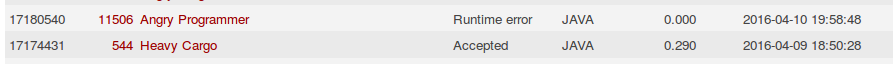
\includegraphics[width=\textwidth]{results}
\newpage

%%%%%%% start Angry Programmer %%%%%%%%%%%%%%%%%%%%%%%%%%%%%%%%%%%%%%%%%%

\section{UVA Problem 11506: Angry Programmer}
\textbf{Background} \\
~\indent You, a programmer of an important software house, have been fired because you
didn't solve an important problem that was assigned to you. You are very furious
and want to take revenge on your boss, breaking the communication between his
computer
and the central server. \\
~\indent The computer of your boss and the central server are in the same network, which
is composed of many machines (computers) and wires linking pairs of those machines.
There is at most one wire between any pair of machines and there can be pairs of
machines without a wire between them. \\
~\indent To accomplish your objective, you can destroy machines and wires, but you can't
destroy neither the computer of your boss nor the central server, because those machines
are monitored by security cameras. You have estimated the cost of blowing up
each machine and the cost of cutting each wire in the network. \\
~\indent You want to determine the minimum cost of interrupting the communication between
your boss' computer and the central server. Two computers $A$ and $B$ can
communicate if there is a sequence of undestroyed machines $x_1,...,x_n$ such that
$x_1 = A, x_n = B$ and $x_i$ is linked with $x_{i+1}$ with an uncut wire (for each $1 \leq i \leq n - 1$). \\ \\
\textbf{Input} \\
The input consists of several test cases. Each test case is represented as follows:
\begin{itemize}
    \item A line with two integers $M$ and $W$ ($2 \leq M \leq 50, 0 \leq W \leq 1000$), representing
    (respectively) the number of machines and the number of wires in the network.
    \item \textbf{M-2} lines, one per machine (different from the boss' machine and the central
    server), containing the following information seperated by spaces:
    \begin{itemize}
        \item An integer $i\ (2 \leq i \leq M-1)$ with the identifier of the machine. Assume
        that the boss' machine has id 1 and that the central server has id $M$.
        \item An integer $c\ (0 \leq c \leq 100000)$ specifying the cost of destroying the machine.
    \end{itemize}
    \item \textbf{W} lines, one per wire, containing the following information separated by spaces:
    \begin{itemize}
        \item Two integers $j$ and $k\ (1 \leq j \textless k \leq M)$ specifying the identifiers of the machines linked by the wire. remember that the wire is bidirectional.
        \item An integer $d (0 \leq d \leq 100000)$ specifying the cost of cutting the wire.
    \end{itemize}
\end{itemize}
The end of the input is specified by a line with the string "0 0". \\
Suppose that the machines have distinct identifiers.

%%%%%%% end Problem %%%%%%%%%%%%%%%%%%%%%%%%%%%%%%%%%%%%%%%%%%%%%%%

\newpage

%%%%%%% Mathematical Formulation %%%%%%%%%%%%%%%%%%%%%%%%%%%%%%%%%%
\subsection{Mathematical Formulation}
Given an input of $M$ machines, $M-2$ of which are potential intermediate nodes
between the boss' computer and the server, and $W$ wires connecting computers $m_i$
and $m_j$ where $0 \leq i \textless j \leq M$, determine the minimum cost to destroy (m + w)
machines and wires where $(0 \leq m \leq M-2, 0 \leq w \leq W)$.

%%%%%%% Algorithm %%%%%%%%%%%%%%%%%%%%%%%%%%%%%%%%%%%%%%%%%%%%%%%%%

\subsection{Solution}
Important Confusing Data Structures:
\begin{itemize}
    \item LinkedList$\textless$FlowEdge$\textgreater$[ ] \textbf{adj} : ~ An adjacency list of all FlowEdges where the
    specified node is the originating node.
\end{itemize}

The main functionality of this algorithm is to implement the Ford Fulkerson min
cut algoritm by first building a flow network and then executingthe algorithm on it.
We represent the network as each machine (index) has its own linked list of Flow
Edges. Each computer has 2 nodes, one as its input and the other as its output. The
only edge that flows out of the input and into the output is the edge connecting the
two such that the input points to the output with edgeweight equivalent to the cost
of destroying that computer; this is the MAX\_INTEGER for the boss' computer and
the server since we cannot destroy these. Since we are given the boss' computer as
"1" and the server as "M" we just let the input for every computer be index = i-1
and their output as index = (i-1)+M for $i \in 1..M$ as described below.

\begin{algorithm}[H]
\caption{Determine index of Computers}
\begin{algorithmic}
    \Procedure{detIndex}{int index, boolean out}
        \If{out}
            return (index - 1) +  m
        \EndIf
        \State return (index - 1)
    \EndProcedure
\end{algorithmic}
\end{algorithm}

Once we do this we have to ensure that the bi-directional rule is accounted for.
So, for each wire connecting computers A and B with cost C, we will connect the
output for A to the input for B with weight C and the output of B to the input of A
with cost C. Once we have built up the entirety of our network we will simply use
the Ford Fulkerson algorithm on the built network and print that out. (As outlined
below)

\begin{algorithm}[H]
\caption{Build the Flow Network from input}
\begin{algorithmic}
    \Procedure{Main}{Scanner input}
        \While{true}
            \State $m, w \gets$ from input
            \If{m == 0 \&\& w == 0}
                break;
            \EndIf
            \If{w == 0}
                \State \Call{print}{0}
                \For{m-2 times}
                    input.\Call{nextLine}{ }
                \EndFor
            \EndIf
            \State $int numV,serverIn \gets$ 2*m, m-1 respectively
            \State $adj[numV] \gets$ initialized
            \State // create computers
            \State adj[0].\Call{add}{FlowEdge(0, m, Integer.MAX\_VALUE)}
            \State adj[serverIn].\Call{add}{FlowEdge(serverIn, numV-1, Integer.MAX\_VALUE)}
            \For{length of m-2}
                \State $int i, c \gets$ index of machine and cost to destroy
                \State $FlowEdge e \gets$ new FlowEdge(i, i+m, c)
                \State adj[i].\Call{add}{e}
            \EndFor
            \State // connect computers to eachother
            \For{length of W}
                \State $int a, b, c \gets$ comp1, comp2, cost to cut wire
                \State $outA, inA \gets$ detIndex(a, true), detIndex(a, false)
                \State $outB, inB \gets$ detIndex(b, true), detIndex(b, false)
                \State $e1, e2 \gets$ FlowEdge(outA, inB, c), FlowEdge(outB, inB)
            \EndFor
            \State \Call{print}{calcMinCut()}
        \EndWhile
    \EndProcedure
\end{algorithmic}
\end{algorithm}

%%%%%%% Correctness %%%%%%%%%%%%%%%%%%%%%%%%%%%%%%%%%%%%%%%%%%%%%%%

\subsection{Correctness}
%%%%%%% PROPOSITION 1 %%%%%%%%%%%%%%%
\begin{proposition}
~ \\ \indent This is the correct flow Network to build which will yeild the min cut.
\end{proposition}

\begin{proof}
~ \\ \indent This is correct because we are using the "flow" of each edge to be the cost of
destroying either a wire or a computer. We account for the fact that if we destroy
a computer, then we will also sever any connection that used this computer as an
intermediate node. We have done this by seperating each computer into an input and
an output node, between which $\exists$ only one connection which has a flow of the cost of
destroying a computer. The bi-directional aspects has us connect the network such
that, for each wire connecting computers A and B with cost C, we will connect the
output for A to the input for B with weight C and the output of B to the input of A
with cost C. Therefore if we sever inA to outA (destroying computer A) B would
no longer be able to use this as an intermedite node since inA no longer has any out
edges and outA is unreachable since its only in edge was just severed.
\end{proof}

%%%%%%% Analysis %%%%%%%%%%%%%%%%%%%%%%%%%%%%%%%%%%%%%%%%%%%%%%%%%%
\subsection{Analysis}
For the following analysis, we will say that we have built a flow network graph with
$V = 2\cdot M$ and $E = M + 2\cdot W$. Our Time and Space analysis will be done with these
variables but can be converted to V $\approx$ M and E $\approx$ (M+W)

%%%%%%% PROPOSITION 1 %%%%%%%%%%%%%%%
\begin{proposition}
\label{numq}
The \underline{space complexity} of this algorithm is \textbf{O(V+E)}
\end{proposition}

\begin{proof}
~ \\ \indent This is due to the fact that all of our data is stored in data structures:
\begin{itemize}
    \item \underline{adj[V]}: Our Flow NetWork $\implies V+E$
    \item \underline{edgeTo[V]}: Used in Ford Fulkerson implementation
\end{itemize}
\begin{center}
    Giving us a space complexity of \textbf{O(V+E)}
\end{center}
\end{proof}

%%%%%%% PROPOSITION 2 %%%%%%%%%%%%%%%
\begin{proposition}
\label{numq}
The \underline{time complexity} of this algorithm is \textbf{O(V+E+MaxFlowValue$\cdot$E)}
\end{proposition}

\begin{proof}
~ \\ \indent This is the case because our algorithm first builds our flow network which
takes V + E time and then implements the Ford Fulkerson Min Cut algorithm which
is synonomous to the Max Flow. This implementation takes MinCutValue$\cdot$E time.
\begin{center}
    Giving us a time complexity of \textbf{O(V+E+MaxFlowValue$\cdot$E)}
\end{center}
\end{proof}

%%%%%%% Example %%%%%%%%%%%%%%%%%%%%%%%%%%%%%%%%%%%%%%%%%%%%%%%%%%%

\subsection{An Example}
\textbf{input} \\
4 4   \\
3 5   \\
2 2   \\
1 2 3 \\
1 3 3 \\
2 4 1 \\
3 4 3 \\
0 0   \\
\\
Now when we run this through our Algorithm we will build first the nodes for the
computers and connect their "ins" to their "outs"
\begin{center}
(boss) $\implies$ 0 $\rightarrow$ 4 with cap = 2.147483647$\cdot10^9$   \\
(server) $\implies$ 3 $\rightarrow$ 7 with cap = 2.147483647$\cdot10^9$  \\
(3 5) $\implies$ 2 $\rightarrow$ 6 with cap = 5.0   \\
(2 2) $\implies$ 1 $\rightarrow$ 5 with cap = 2.0
\end{center}

\noindent Next we build the wire connections:

\begin{center}
(1 2 3) $\implies$ 4 $\rightarrow$ 1 with cap = 3.0 \\
convex $\implies$ 5 $\rightarrow$ 0 with cap = 3.0  \\ ~ \\
(1 3 3) $\implies$ 4 $\rightarrow$ 2 with cap = 3.0 \\
convex $\implies$ 6 $\rightarrow$ 0 with cap = 3.0  \\ ~ \\
(2 4 1) $\implies$ 5 $\rightarrow$ 3 with cap = 1.0 \\
convex $\implies$ 7 $\rightarrow$ 1 with cap = 1.0  \\ ~ \\
(3 4 3) $\implies$ 6 $\rightarrow$ 3 with cap = 3.0 \\
convex $\implies$ 7 $\rightarrow$ 2 with cap = 3.0
\end{center}

Then when we calculate the mincut value we get 4!

%%%%%%% end Angry Programmer %%%%%%%%%%%%%%%%%%%%%%%%%%%%%%%%%%%%%%%%%%%
\newpage
%%%%%%% start Heavy Cargo %%%%%%%%%%%%%%%%%%%%%%%%%%%%%%%%%%%%%%%%%%

\section{UVA Problem 544: Heavy Cargo}
\textbf{Background} \\
~\indent  Big Johnsson Trucks Inc. is a company specialized in manufacturing big trucks.
Their latest model, the Godzilla V12 , is so big that the amount of cargo you can
transport with it is never limited by the truck itself. It is only limited by the weight
restrictions that apply for the roads along the path you want to drive. \\
\indent Given start and destination city, your job is to determine the maximum load of
the Godzilla V12 so that there still exists a path between the two specified cities. \\
\\
\textbf{Input} \\
\indent The input file will contain one or more test cases. The first line of each test case
will contain two integers: the number of cities $n\ (2 \leq n \leq 200)$ and the number of
road segments $r\ (1 \leq r \leq 19900)$ making up the street network. \\
\indent Then $r$ lines will follow, each one describing one road segment by naming the two
cities connected by the segment and giving the weight limit for trucks that use this
segment. Names are not longer than 30 characters and do not contain white-space
characters. Weight limits are integers $\in (0, 10000)$. Roads can always be travelled in
both directions. \\
\indent The last line of the test case contains two city names: start and destination. \\
\indent Input will be terminated by two values of 0 for $n$ and $r$. \\
\\
\textbf{Output} \\
\indent For each test case, print three lines:
\begin{itemize}
    \item a line saying "Scenario \#x" where $x$ is the number of the test case
    \item a line saying "y tons" where $y$ is the maximum possible load
    \item a blank line
\end{itemize}

%%%%%%% end Problem %%%%%%%%%%%%%%%%%%%%%%%%%%%%%%%%%%%%%%%%%%%%%%%

\newpage

%%%%%%% Mathematical Formulation %%%%%%%%%%%%%%%%%%%%%%%%%%%%%%%%%%
\subsection{Mathematical Formulation}
Given an input of $n$ cities, $c_1, c_2,..., c_n$, and $r$ roads with loads $l_1, l_2,..., l_r$ which connect
cities $c_i\ and\ c_j,\ 1 \leq i,j \leq r$, we will determine the maximum load that can be transported
from the specified cities ($a$ to $b$).

%%%%%%% Algorithm %%%%%%%%%%%%%%%%%%%%%%%%%%%%%%%%%%%%%%%%%%%%%%%%%

\subsection{Solution}
Important and potentially confusing data structures:
\begin{itemize}
    \item HashMap$\textless$String, Integer$\textgreater$ \textbf{cityIndex} : keeps track of the index associated
    with each city.
    \item int[n][n] \textbf{load} : ~ each element load[i][j] stores the highest constraining load that
    each road connecting city i and j.
    \item int[n] \textbf{curSet} : ~ stores the current row/column that we will add together for
    the Floyd-Warshall implementation.
    \item int[n][n] \textbf{l\_i} : ~ corresponding row/column sum that is calculated in each sub
    situation during the Floyd-Warshall algorithm.
\end{itemize}

The main functionality of this algorithm is an adapted Floyd-Warshall implementation
where we first build up our cityIndex HashMap and our load[ ][ ] which stores
the max load that each road can take between city "a" and city "b".

\begin{algorithm}[H]
\caption{Set-Up}
\begin{algorithmic}
    \Procedure{build}{Scanner in}
        \State $int senario \gets$ 0
        \While{true}
            \State $n, r \gets$ number of cities and number of roads from $in$
            \If{n == 0 and r == 0}
                break;
            \EndIf
            \State $load[n][n] and cityIndex \gets$ initialized
            \State $int lastIndex \gets$ 0
            \For{$i \in 0..(r-1)$}
                \State If not in hashmap put in.
                \State $int a, b \gets$ index of the two connected cities from $cityIndex$
                \State $int curLoad \gets$ the load specified by the file
                \State $load[a][b], load[b][a] \gets$ curLoad;
            \EndFor
            \State \Call{flyodWarshall}{load} // see Algorithm 2
            \State $int a, b \gets$ index of the two cities want to connect from $cityIndex$
            \State \Call{print}{load[a][b]}
        \EndWhile
    \EndProcedure
\end{algorithmic}
\end{algorithm}


The main difference comes from our rules, instead of using the rule:
\[ load(i, j, k) = \textbf{min}
\begin{cases}
    load(i, j, k-1) \\
    load(i, k, k-1) + load(k, j, k-1)
\end{cases}
\]
where i, j are the the correspoding cities i and j and i = j $\implies$ load(i,j,k) = 0 $\forall\ k$, we have
\[ load(i, j, k) = \textbf{max}
\begin{cases}
    load(i, j, k-1) \\
    load(i, k, k-1) + load(k, j, k-1)
\end{cases}
\]
One thing to note here is that we will be representing the distances seen so far in our
2-D array $load$ array. When implementing this the things to keep in mind are that
elements load[a][b] = load[b][a] always.

\begin{algorithm}[H]
\caption{Floyd-Warshall Implementation}
\begin{algorithmic}
    \Procedure{floydWarshall}{int[ ][ ] load}
        \State $curSet, l\_i \gets$ initialized
        \For{$i \in 0..(n-1)$}
            \For{$k \in 0..(n-1)$}
                \State $curSet[k] \gets$ load[i][k]
            \EndFor
            \State // build l\_i
            \For{$row \in 0..(n-1)$}
                \For{$col \in 0..(n-1)$}
                    \If{row == col}
                        continue;
                    \EndIf
                    \State $l\_i[row][col] \gets$ Math.\Call{min}{curSet[row], curSet[col]};
                \EndFor
            \EndFor
            \State // do dynamic step
            \For{$row \in 0..(n-1)$}
                \For{$col \in 0..(n-1)$}
                    \If{row == col}
                        continue;
                    \EndIf
                    \State $load[row][col] \gets$ Math.\Call{max}{load[row][col], l\_i[row][col]};
                \EndFor
            \EndFor
        \EndFor
    \EndProcedure
\end{algorithmic}
\end{algorithm}

%%%%%%% Correctness %%%%%%%%%%%%%%%%%%%%%%%%%%%%%%%%%%%%%%%%%%%%%%%

\subsection{Correctness}
%%%%%%% PROPOSITION 1 %%%%%%%%%%%%%%%
\begin{proposition}
~ \\ \indent Our adapted Floyd-Warshall Shortest Path Distance algorithm to a Floyd-Warshall
Highest Load algorithm sufficiently solves the problem.
\end{proposition}

\begin{proof}
~ \\ \indent In class we prooved that the Floyd-Warshall Shortest Path Distance algorithm
will determine the shortest path between two nodes given a "graph" with the edge
weights being the distance between two nodes. Now the dynamic algorithm rule that
we use to build this solution is expressed as:
\[ dist(i, j, k) = \textbf{min}
\begin{cases}
    dist(i, j, k-1) \\
    dist(i, k, k-1) + dist(k, j, k-1)
\end{cases}
\]
\[
where,\ dist(i, j, 0) =
\begin{cases}
    w_{i,j}\ if\ (i, j) \in E \\
    \infty\ if\ (i, j) \notin E \\
    0\ if\ i = j
\end{cases}
\]
Such that $w_{i,j}$ is the weight between nodes $i$ and $j$ and $E$ is the set of all edges. Now
we adapt this such that $E$ is all roads, $w_{i,j}$ is the load of each road between cities $i$
and $j$. Therefore we are no longer looking for distances, but loads $\implies dist \rightarrow load$
and instead of finding the min we are looking for the max. Therefore, we have the
new formulation:
\[ load(i, j, k) = \textbf{max}
\begin{cases}
    load(i, j, k-1) \\
    load(i, k, k-1) + load(k, j, k-1)
\end{cases}
\]
Which is the algorithm which we have implemented. Since this is the only difference with
the original, we can say that this is sufficient to solve the given problem.
\end{proof}


%%%%%%% Analysis %%%%%%%%%%%%%%%%%%%%%%%%%%%%%%%%%%%%%%%%%%%%%%%%%%
\subsection{Analysis}
For the following analysis, we will say that $N$ is the number of cities that are given
to us. We note here that all of the analysis is dependent on the number of cities and
not the number of roads. This is due to the fact that the roads are being represented
through our load[ ][ ] which is dependent on $N$ already.

%%%%%%% PROPOSITION 1 %%%%%%%%%%%%%%%
\begin{proposition}
\label{numq}
The \underline{space complexity} of this algorithm is \textbf{O(N$^2$)}
\end{proposition}

\begin{proof}
~ \\ \indent This is due to the fact that all of our data is stored in data structures:
\begin{itemize}
     \item HashMap$\textless$String, Integer$\textgreater$ \textbf{cityIndex} : stores indexes of all cities $\implies N$
    \item int[n][n] \textbf{load} : ~ stores the distances from cities a to b $\implies N^2$
    \item int[n] \textbf{curSet} : ~ stores the row/column distances that will be used to calculate l\_i $\implies N$
    \item int[n][n] \textbf{l\_i} : ~ stores the calculated distances from cities a to b ($N^2$) from  $curSet$ $\implies N^2$
    \item \underline{cause}: reason $\implies complexity$
\end{itemize}
At any point in time, there will exist at most one of each of these data structures $\implies$ $2\cdot N^2 + 2\cdot N$
\begin{center}
    $\therefore$ Giving us a space complexity of \textbf{O(N$^2$)}
\end{center}
\end{proof}

%%%%%%% PROPOSITION 2 %%%%%%%%%%%%%%%
\begin{proposition}
\label{numq}
The \underline{time complexity} of this algorithm is \textbf{O(N$^3$)}
\end{proposition}

\begin{proof}
This is the case because our algorithm is just the adjusted Floyd-Warshall
Algorithm which builds $N$, $N$x$N$ matricies. At each step, $n\ s.t.\ 1 \leq n \leq N$ we are
computing the $N$x$N$ matrix in linear time ($N^2$) and somparing each element to an
existing $N$x$N$ graph which is also done in linear time. Therefore we are going through
$N^2$ operations $N$ times.
\begin{center}
    $\therefore$ Giving us a time complexity of \textbf{O(N$^3$)}
\end{center}
\end{proof}

%%%%%%% Example %%%%%%%%%%%%%%%%%%%%%%%%%%%%%%%%%%%%%%%%%%%%%%%%%%%

\subsection{An Example}
Given the input: \\
4 3     \\
K S 100 \\
S U 80  \\
U M 120 \\
K M     \\
We build our initial matrix load[4][4]:
\[  load =
\begin{bmatrix}
    \textbf{0}   & \textbf{100} & \textbf{0}   & \textbf{0}   \\
    \textbf{100} & 0   & 80  & 0   \\
    \textbf{0}   & 80  & 0   & 120 \\
    \textbf{0}   & 0   & 120 & 0
\end{bmatrix}
\]
And we begin our Floyd-Warshall algorithm by computing l\_i with the rows bolded
above to produce (the altered load elements have been underlined):
\[  l\_1 =
\begin{bmatrix}
    0   & 0   & 0   & 0   \\
    0   & 0   & 0   & 0   \\
    0   & 0   & 0   & 0   \\
    0   & 0   & 0   & 0
\end{bmatrix}
\implies load =
\begin{bmatrix}
    0   & \textbf{100} & 0   & 0   \\
    \textbf{100} & \textbf{0}   & \textbf{80}  & \textbf{0}   \\
    0   & \textbf{80}  & 0   & 120 \\
    0   & \textbf{0}   & 120 & 0
\end{bmatrix}
\]
continuing computing l\_i with the rows bolded above to produce:
\[  l\_2 =
\begin{bmatrix}
    0   & 0   & 80   & 0   \\
    0   & 0   & 0   & 0   \\
    80   & 0   & 0   & 0   \\
    0   & 0   & 0   & 0
\end{bmatrix}
\implies load =
\begin{bmatrix}
    0   & 100 & \textbf{\underline{80}}  & 0   \\
    100 & 0   & \textbf{80}  & 0   \\
    \textbf{\underline{80}}  & \textbf{80}  & \textbf{0}   & \textbf{120} \\
    0   & 0   & \textbf{120} & 0
\end{bmatrix}
\]
continuing computing l\_i with the rows bolded above to produce:
\[  l\_3 =
\begin{bmatrix}
    0   & 80   & 0   & 80   \\
    80   & 0   & 0   & 80   \\
    0   & 0   & 0   & 0   \\
    80   & 80   & 0   & 0
\end{bmatrix}
\implies load =
\begin{bmatrix}
    0   & 100 & 80  & \textbf{\underline{80}}   \\
    100 & 0   & 80  & \textbf{\underline{80}}   \\
    80  & 80  & 0   & \textbf{120} \\
    \textbf{\underline{80}}  & \textbf{\underline{80}}  & \textbf{120} & \textbf{0}
\end{bmatrix}
\]
and computing the final l\_i with the rows bolded above to produce:
\[  l\_3 =
\begin{bmatrix}
    0   & 80   & 80   & 0   \\
    80   & 0   & 80   & 0   \\
    80   & 80   & 0   & 0   \\
    0   & 0   & 0   & 0
\end{bmatrix}
\implies load =
\begin{bmatrix}
    0   & 100 & 80  & 80   \\
    100 & 0   & 80  & 80   \\
    \textbf{80}  & 80  & 0   & 120 \\
    80  & 80  & 120 & 0
\end{bmatrix}
\]
Therefore since K correlates with index 0 and M with index 3, the maximum load is
then load[0][3] = 80 (as bolded above)


%%%%%%% end Heavy Cargo %%%%%%%%%%%%%%%%%%%%%%%%%%%%%%%%%%%%%%%%%%%
\newpage
%%%%%%% start ROTC %%%%%%%%%%%%%%%%%%%%%%%%%%%%%%%%%%%%%%%%%%

\section{Book 6.16: ROTC}
\textbf{Background} \\
~\indent There are many sunny days in Ithaca, New York; but this year, as it happens, the
spring ROTC picnic at Cornell has fallen on a rainy day. The ranking officer decides
to postpone the picnic and must notify everyone by phone. Here is the mechanism
she uses to do this. \\
~\indent Each ROTC person on campus except the ranking officer reports to a unique
$superior\ officer$. Thus the reporting hierarchy can be described by a tree $T$, rooted
at the ranking officer, in which each other node $v$ has a parent node $u$ equal to his or
her superior officer. Conversely, we will call $v$ a $direct\ subordinate$ of $u$. \\
~\indent To notify everyone of the postponement, the ranking officer first calls each of her
direct subordinates, one at a time. As soon as each subordinate gets the phone call,
he or she must notify each of his or her direct subordinates, one at a time. The
process continues this way until everyone has been notified. Note that each person in
this process can only call direct subordinates on the phone. \\
~\indent We can picture this process as being divided into rounds. In one round, each
person who has already learned of the postponement can call one of his or her direct
subordinates on the phone. The number of rounds it takes for everyone to be notified
depends on the sequence in which each person calls their direct subordinates. \\
~\indent Give an efficient algorithm that determines the minimum number of rounds needed
for everyone to be notified, and outputs a sequence of phone calls that achieves this
minimum number of rounds.

%%%%%%% end Problem %%%%%%%%%%%%%%%%%%%%%%%%%%%%%%%%%%%%%%%%%%%%%%%

\newpage

%%%%%%% Mathematical Formulation %%%%%%%%%%%%%%%%%%%%%%%%%%%%%%%%%%
\subsection{Mathematical Formulation}
Given an input of the tree T with $n$ nodes in total and depth of $d$. Let the most
number of direct subordinates (children) any one officer (parent) has be expressed as
$c$. We will determine least number of calls needed to reach every node of the tree as
well as the order in which to acheive this.

%%%%%%% Algorithm %%%%%%%%%%%%%%%%%%%%%%%%%%%%%%%%%%%%%%%%%%%%%%%%%

\subsection{Solution}
This algorithm begin by doing a by-level bottom up traversal. As it traverses, it will
assign values to each node based off its children. The way it does this is first sorting
all of its children from highest value to lowest and such that $v_0 \geq v_1 \geq ... \geq v_{n-1}$ for
a node with $n$ children, then saying:
\[ value =
\begin{cases}
    0\ if\ no\ children \\
    max_{i \in 0..(n-1)}\ (child_{i}value + 1 + i)\ else
\end{cases}
\]
With this we will develope our values and when we reach the top level ($n$), its value
will be the least number of calls needed to be made. Our path to take then is to call
the open value node from each seen node.

\begin{algorithm}[H]
\caption{Fill out Tree and get num Calls}
\begin{algorithmic}
    \Procedure{getNumCalls}{Tree T}
        \For{$level \in 1..d$}
            \For{$node \in T.level(level)$}
                \State int value = 0
                \If{node.hasChildren}
                    \State children.inverseSort
                    \State int i = 0
                    \For{$child \in children$}
                        \State childV = child.value + 1 + (i++)
                        \State value = max(value, childV)
                    \EndFor
                \EndIf
                \State node.\Call{setValue}{value}
            \EndFor
        \EndFor
        \State print(root.value)  // least num calls
        \State \Call{traverse}{T} // T has all values filled out and inverse sorted
    \EndProcedure
\end{algorithmic}
\end{algorithm}


%%%%%%% Correctness %%%%%%%%%%%%%%%%%%%%%%%%%%%%%%%%%%%%%%%%%%%%%%%
\newpage
\subsection{Correctness}
%%%%%%% PROPOSITION 1 %%%%%%%%%%%%%%%
\begin{proposition}
~ \\ \indent This algorithm will determine the correct minimum number of calls.
\end{proposition}

\begin{proof}
~ \\ \indent We do this by construction. We observe that doing a bottom up traversal we can
see that as long as the children have the correct value, then the parent will be able to
calculate the correct value. When I say value of a node I am referring to the number
of calls required to fully reach the subtree rooted at this node, assuming the node has
already been reached. $\implies$ if the node is a leaf, its value = 0. Therefore when we have
a node with a single leaf as a child, $\implies$ will take the number of calls that the
leaf will make, 0, + 1 because it has to call the leaf. Now if there are multiple children,
k of them, and all of them are leaves we will note that we cannot call multiple leaves at
the same time, therefore the number of calls that this node will have to make is $n$ and
its value will also be n since each of the nodes must make 0 calls. \\
\indent Now lets change it such that each of the children have thier own value $v_1,...,v_n$
we note that it will always be most efficient to call the children with more calls to make
first, therefore let us inverse-sort them based off of their values s.t. $v_1\geq...\geq v_n$
Now we can create a $value$ variable and set it equal to cost of calling $c_1$ which is
$v_1 + 1$ beacause we have to call the node itself. We will then check to see if the cost of calling
$c_2$ exceeds that of $c_1$ as in is cost of calling $c_2$ second $\textgreater$ cost of calling
$c_1$ first? i.e. $value = max(value, v_2 + 1 + 1)$ since it cost 0 to call first, 1
to call second , 2 to call third, etc. We will then continue with this letting
$value = max_{i \in 1..(n)}\ (child_{i}value + 1 + (i-1))$ \\
\indent After we have done this for every node (building from bottom $\rightarrow$ up), we
just ask for the value of the root which will give us the minimum number of calls we
have to make to reach everyone.
\end{proof}


%%%%%%% Analysis %%%%%%%%%%%%%%%%%%%%%%%%%%%%%%%%%%%%%%%%%%%%%%%%%%
\subsection{Analysis}

%%%%%%% PROPOSITION 1 %%%%%%%%%%%%%%%
\begin{proposition}
\label{numq}
The \underline{space complexity} of this algorithm is \textbf{O(size(T))}
\end{proposition}

\begin{proof}
~ \\ \indent This is due to the fact that all of our data is stored in the tree itself:
\end{proof}

%%%%%%% PROPOSITION 2 %%%%%%%%%%%%%%%
\begin{proposition}
\label{numq}
The \underline{time complexity} of this algorithm is \textbf{O(N$\cdot$n$^{\ast}\cdot$log(n$^{\ast}$))}
\end{proposition}

\begin{proof}
~ \\ \indent Let us define the average number of children every node has as $n^{\ast} \implies$ the
cost to sort will be $n^{\ast}\cdot log(n^{\ast})$ now since we have to sort for each node, N times
$\implies N\cdot n^{\ast}\cdot log(n^{\ast})$ Note here though that $n^{\ast}$ is likely to be a low
number when compared to $N$.
\end{proof}


%%%%%%% end ROTC %%%%%%%%%%%%%%%%%%%%%%%%%%%%%%%%%%%%%%%%%%%

%%%%%%% end Solution %%%%%%%%%%%%%%%%%%%%%%%%%%%%%%%%%%%%%%%%%%%%%%

\end{document}